\subsection{UC31 - Visualizzazione errore posizione suddivisione non valida}
\begin{figure}[H]
  \centering
  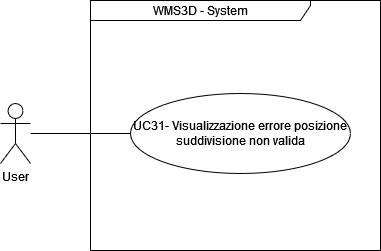
\includegraphics[width=0.5\textwidth]{UC_diagrams_28-32/UC31_sys.drawio.png}
  \caption{Diagramma UML UC31 - Visualizzazione errore posizione suddivisione non valida}
\end{figure}
\begin{itemize}
    \item \textbf{Attori:} User.
    \item \textbf{Pre-condizione:} L'utente sceglie una posizione per la suddivisione che eccede i confini del magazzino o che interseca altre suddivisioni.
    \item \textbf{Post-condizione:} L'utente visualizza un messaggio d'errore e il posizionamento non viene permesso.
    \item \textbf{Scenario Principale:} L'utente visualizza un messaggio informativo sull'errore. L'utente dovrà cambiare posizionamento.
    \item \textbf{Generalizzazioni:} -
    \item \textbf{Estensioni:} -
\end{itemize}